
\par\noindent\textbf{关于 (7.2.280.1)。}
首先将同伦 (7.2.280.1) 分解为两个同伦的复合。
以下用 $j$ 表示各种包含映射的同伦逆。
例如，
$j\colon C(L'_0,(\lambda_0,\lambda'_0))
\to C(L'_0,\lambda'_0)$
是包含映射
$C(L'_0,\lambda'_0)\to
C(L'_0,(\lambda_0,\lambda'_0))$
的同伦逆。
以下始终假设 $j$ 在
$C(L'_0,\lambda'_0)$ 等子复形上为恒等映射。

注意，(7.2.280.1) 是如下两个同伦的复合：
\begin{equation}
\begin{aligned}
\mathfrak g^{\phi'}\circ\mathfrak g^{\psi_{0,s_0}}
&=j\circ\mathfrak f^{\phi'}\circ j\circ
\mathfrak f^{\psi_{0,s_0}}\\
&\sim j\circ\mathfrak f^{\phi'}_{\mathrm{ext},s=s_0}
\circ\mathfrak f^{\psi_{0,s_0}},
\end{aligned}
\tag{7.2.298.1}\label{eq:7-2-298-1}
\end{equation}
\begin{equation}
j\circ\mathfrak f^{\phi'}_{\mathrm{ext},s=s_0}
\circ\mathfrak f^{\psi_{0,s_0}}
\sim j\circ\mathfrak f^{\phi'\circ\psi_{0,s_0}}
=\mathfrak g^{\phi'\circ\psi_{0,s_0}}.
\tag{7.2.298.2}\label{eq:7-2-298-2}
\end{equation}
映射 $\mathfrak f^{\phi'}_{\mathrm{ext},s=s_0}$
将在后文定义。

先讨论同伦 (7.2.298.1) 及其以 $s$ 为参数的版本。

\begin{lemma}{7.2.299}\label{lem:7-2-299}
存在 $L'_1$ 的光滑奇异链复形的子复形
\[
C_a^{s=s_0}(L'_1,((\lambda_0,\lambda'_0),\lambda'_1)),
\]
其上带有滤过 $A_{n',K'}$ 结构；
还存在滤过 $A_{n,K}$ 同态
\[
\mathfrak f^{\phi'}_{\mathrm{ext},s=s_0}\colon
C(L'_0,(\lambda_0,\lambda'_0))
\longrightarrow
C_a^{s=s_0}(L'_1,((\lambda_0,\lambda'_0),\lambda'_1)).
\]
包含映射\translatornote{原书在此把左端写作
$C(L'_1,(\lambda_1,\lambda'_1))$；
图式 7.2.17 及后续引理 7.2.300
均使用 $C(L'_1,(\lambda'_0,\lambda'_1))$，
且未假设 $\lambda_1=\lambda'_0$，
这里依相邻包含链定型。}
\[
C(L'_1,(\lambda'_0,\lambda'_1))
\longrightarrow
C_a^{s=s_0}(L'_1,((\lambda_0,\lambda'_0),\lambda'_1))
\]
是同伦等价，且图式~\ref{diag:7-2-17} 交换。

\par\medskip\noindent\begin{minipage}{\textwidth}
\centering
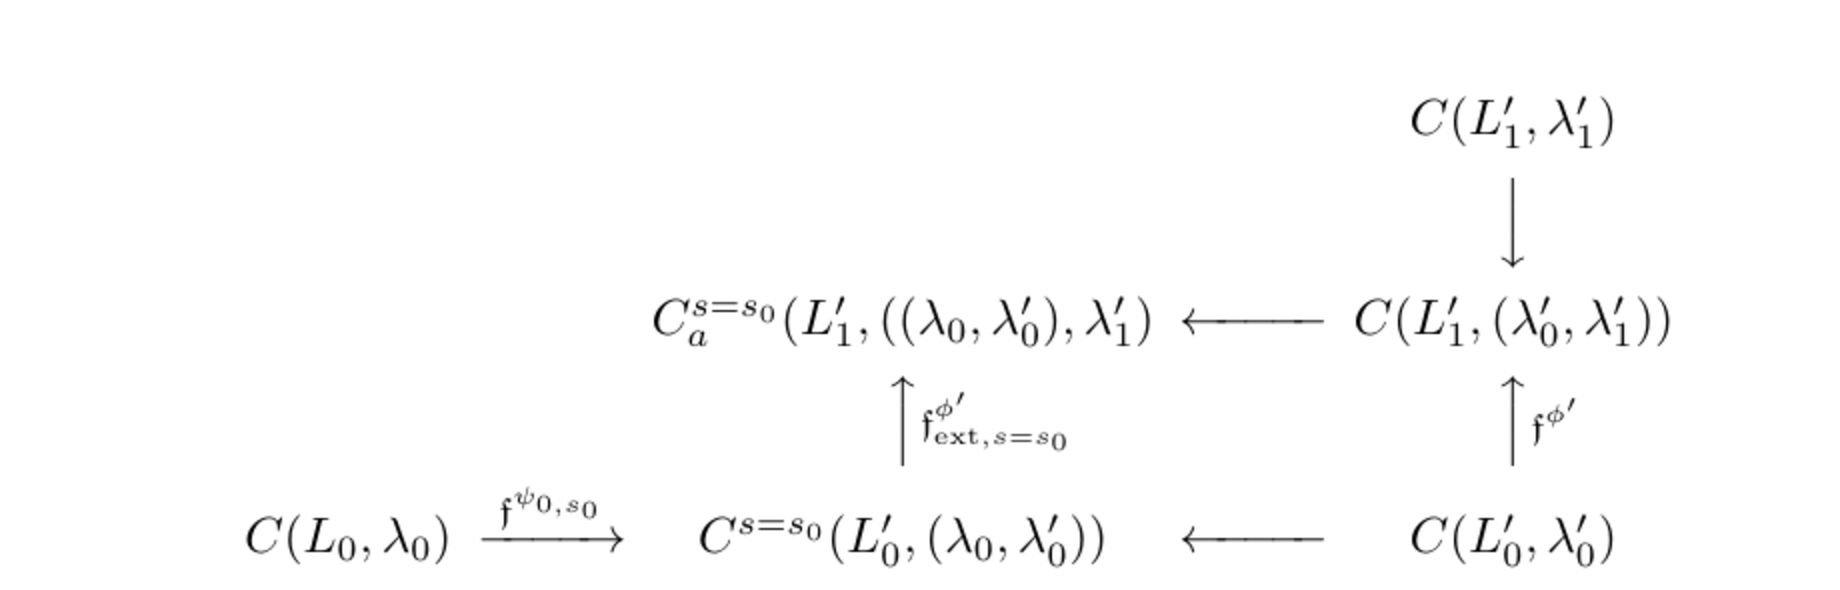
\includegraphics[width=\textwidth]{chapters/ch07-transversality/figures/phys-558-diagram-7-2-17-math-crop.png}
\par{\renewcommand{\thefigure}{7.2.17}\refstepcounter{figure}
\normalfont\bfseries 图式~\thefigure\label{diag:7-2-17}}
\end{minipage}\par\medskip
\end{lemma}

证明与第 7.2.9 小节的论证相同
（亦见第 4.6.3 小节末尾）。

须指出，图式~\ref{diag:7-2-17}
是严格交换的，而非仅在同伦意义下交换。
这一点对后面的论证很重要，
因为我们需要建立若干严格等式。
不过，若将其中箭头反向
（即以 $j$ 代替包含映射），
图式便只在滤过 $A_{n,K}$ 同伦意义下交换。
这个同伦正是 (7.2.298.1)；
后文还会回到这一点。

现在构造图式~\ref{diag:7-2-17}
的 $s$ 参数化版本。
